\documentclass[a4paper,12pt]{article}

 \addtolength{\oddsidemargin}{-.5in}
\addtolength{\evensidemargin}{-.5in}
\addtolength{\textwidth}{1.0in}
\addtolength{\topmargin}{-.5in}
\addtolength{\textheight}{1.0in}


\usepackage{cite}

\usepackage{graphicx}
\usepackage{amsmath}
\usepackage{amssymb}
\usepackage{amsthm}
\usepackage{xcolor}
\usepackage{color}
\usepackage{bbding}
\usepackage{algorithm}
\usepackage[noend]{algpseudocode}
\newtheorem{theorem}{Theorem}
\newtheorem{corollary}{Corollary}

\begin{document}

\title{Group 4: The Kaczmarz Algorithm}
\author{Wei Deng, Nicole Eikmeier, Nate Veldt, and Xiaokai Yuan}
\maketitle{}


\section{Introduction}
Project Objective:

Given a large sparse linear system $Ax = f$, of order $n = 10^6$ that can be effectively reduced to a banded matrix using the reordering scheme ``reverse Cuthill-McKee", use the method of Row Projection, accelerated via the Conjugate Algorithm to yield a parallel solver. Compare the robustness and parallel scalability/speed with preconditioned Krylov subspace methods preconditioned via approximate LU-factorization.

\vspace{.2in}

The Kaczmarz Algorithm is a row projection method which is equivalent to solving $AA^Ty = f$ using the Gauss-Siedel iteration, with $x = A^Ty$. In Kaczmarz we consider each equation as a hyperplane:
$$S_i=\{x:A_ix-b_i=0\}$$ for $i=1,2,...$, where $A_i$ and $b_i$ are $i$th row of matrix $A$ and vector $b$. So the problem is transformed into finding the coordinates of the point of intersection of these hyperplanes.  See figure \ref{fig:ClassKacz} for a visualization of the problem.

\begin{figure}[htbp]
\begin{centering}
%\begin{minipage}[b]{0.8\linewidth}
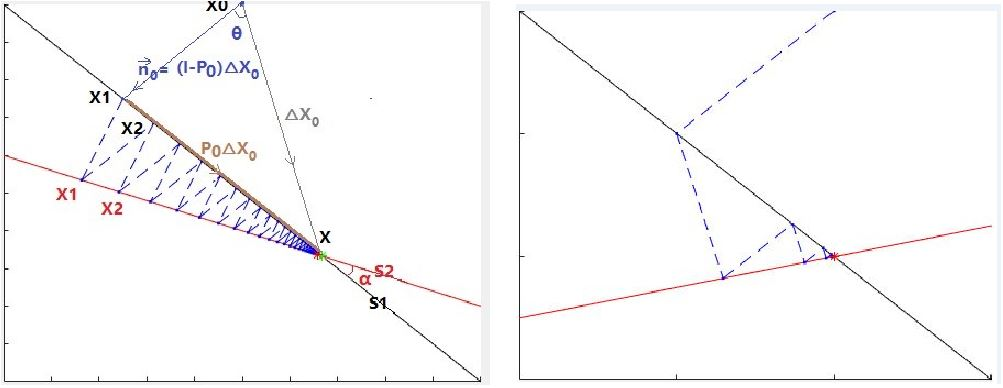
\includegraphics[width=5in]{Images/Classical_Kaczmarz}
\caption{2-Partition Case of the Kaczmarz Algorithm}
\label{fig:ClassKacz}
%\end{minipage}
\end{centering}
\end{figure}

From this basic idea we use symmetrization and acceleration via the CG method to improve the procedure. The details will be given carefully in the following sections.




\section{Implementation}


%------------------------------------------------
%------------------------------------------------
% REVERSE CUTHILL-MCKEE
%------------------------------------------------
%------------------------------------------------

\subsection{Reverse Cuthill-McKee and the Woodbury Formula}
The first step in our implementation is to transform the sparse matrix $A$ to a banded form using Reverse Cuthill-McKee. We can perform a symmetric permutation with matrix $P$ so that $P^TAP$ is banded. In figure \ref{fig:v3}, we see the result from Matlab of Reverse Cuthill Mckee on the stomach data set. The band size is nice and small.

%\begin{figure}[ht]
%\centering
%\begin{minipage}[b]{0.45\linewidth}
%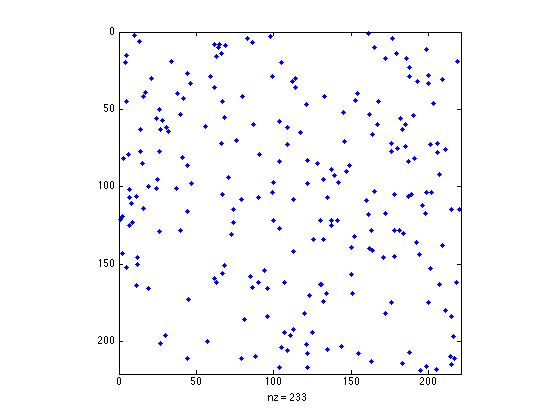
\includegraphics[width=2in]{Images/SparseA.jpg}
%\caption{$A$ sparse, non-symmetric}
%\end{minipage}
%\quad
%\begin{minipage}[b]{0.45\linewidth}
%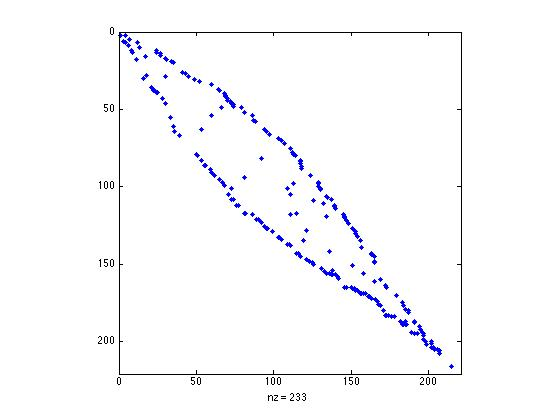
\includegraphics[width=2in]{Images/Arcm.jpg}
%\caption{$P^TAP$ (banded)}
%\label{fig:banded}
%\end{minipage}
%\end{figure}

\begin{figure}[ht]
\centering
\begin{minipage}[b]{0.45\linewidth}
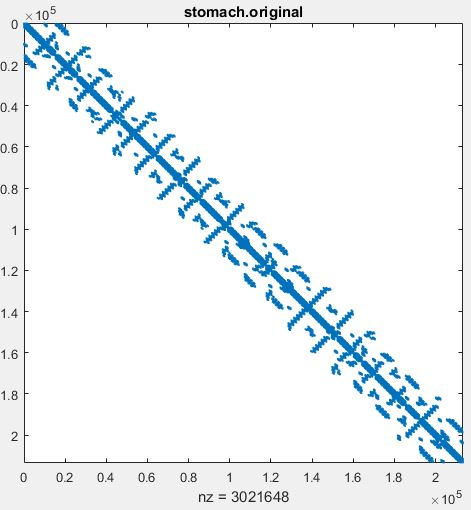
\includegraphics[width=2in]{Images/SparseA_v5.jpg}
\caption{$A$ sparse, non-symmetric}
\label{fig:v5}
\end{minipage}
\quad
\begin{minipage}[b]{0.45\linewidth}
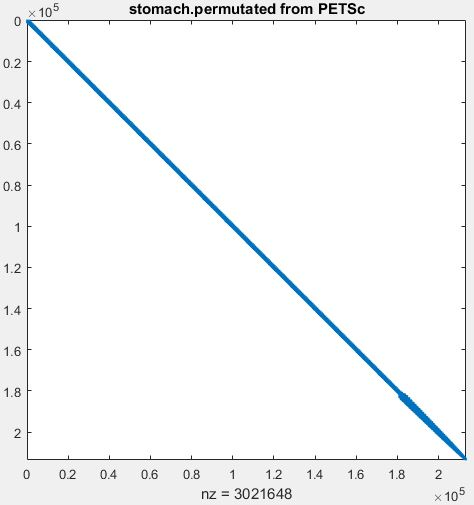
\includegraphics[width=2in]{Images/Arcm_v3.jpg}
\caption{$P^TAP$ (banded)}
\label{fig:v3}
\end{minipage}
\end{figure}

For some problems the bandwidth could be too large after using Reverse Cuthill Mckee. See for example figure \ref{fig:approxbanded}, where we see the result of RCM on the lns$\_$131 data set, again in Matlab.  If this is the case, instead we could choose $P$ so that $P^TAP$ is narrow banded plus a low rank matrix. See figure \ref{fig:woodbury}. 

\begin{figure}[ht]
\centering
\begin{minipage}[b]{0.45\linewidth}
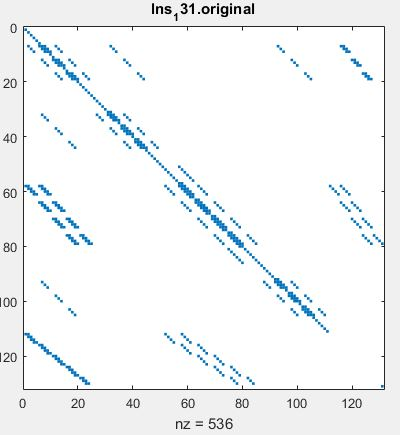
\includegraphics[width=2in]{Images/SparseA_v4.jpg}
\caption{$A$ is sparse and non-symmetric}
\label{sparseA}
\end{minipage}
\quad
\begin{minipage}[b]{0.45\linewidth}
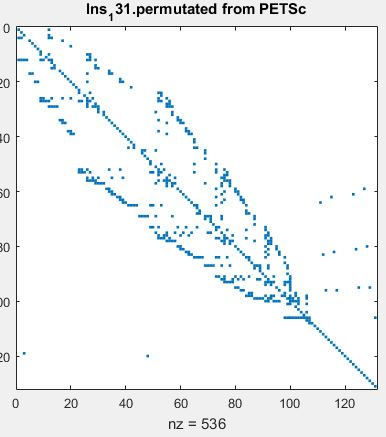
\includegraphics[width=2in]{Images/ApproxBanded_v2.jpg}
\caption{$P^TAP$ narrow band+low rank}
\label{fig:approxbanded}
\end{minipage}
\end{figure}


%\begin{figure}[ht]
%\centering
%\begin{minipage}[b]{0.45\linewidth}
%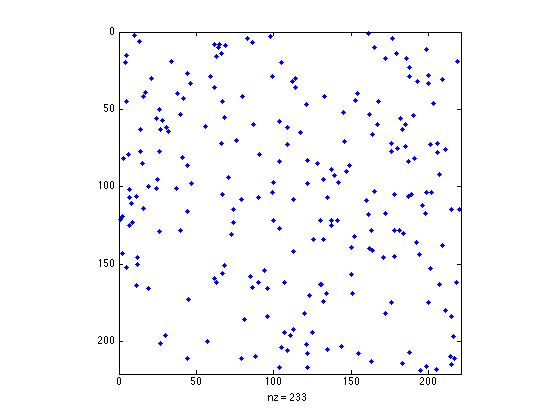
\includegraphics[width=2in]{Images/SparseA.jpg}
%\caption{$A$ is sparse and non-symmetric}
%\end{minipage}
%\quad
%\begin{minipage}[b]{0.45\linewidth}
%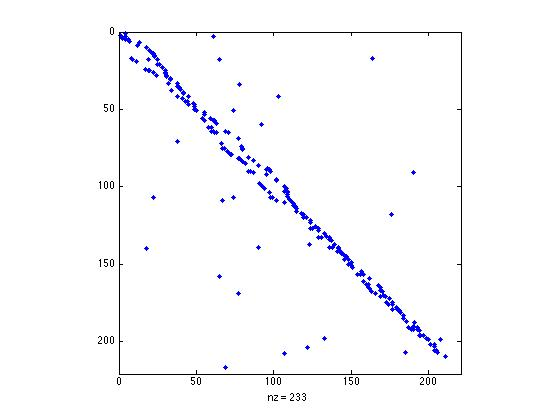
\includegraphics[width=2in]{Images/ApproxBanded.jpg}
%\caption{$P^TAP$ narrow band + low rank}
%\end{minipage}
%\label{fig:bandedplus}
%\end{figure}

\begin{figure}[htbp] %  figure placement: here, top, bottom, or page
   \centering
   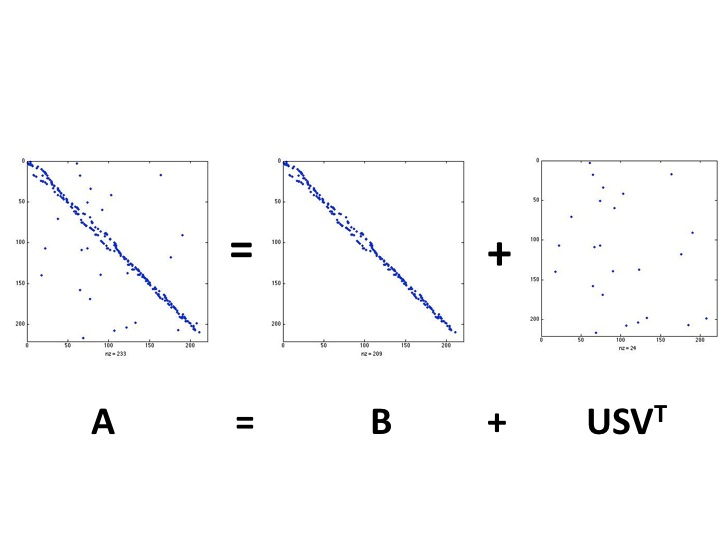
\includegraphics[trim = 5mm 30mm 0mm 40mm, clip, width=4in]{Images/Slide1.jpg}
    \caption{Breaking up $A$ into a banded matrix plus a low rank matrix}
    \label{fig:woodbury}
\end{figure}

In this case we use the Woodbury Formula to solve $Ax = b$. Recall first that $ Ax = b$  implies $x = A^{-1} b$. Then,
%\begin{block}{Woodbury Formula}
\begin{align*}
A^{-1} &= (B - USV^T)^{-1}\\
	  &= B^{-1} - B^{-1}UTV^TB^{-1}
\end{align*}
where $T = (V^TB^{-1}U - S^{-1})^{-1}$. And 
%\end{block}
\begin{align*}
x &= A^{-1}b\\
  &= {\bf B^{-1} b} - B^{-1}UTV^T {\bf B^{-1} b} \\
   &= {\bf a} - B^{-1}UT(V^T {\bf a}) \\
   &= {\bf a} - B^{-1}UT {\bf c}  \hspace{.5cm} \mbox{( solve ($V^TB^{-1}U-S^{-1}) \textbf{d} = \textbf{c}$)}\\
   &= {\bf a} - B^{-1}U\textbf{d}\\
   &= {\bf a} - B^{-1}\textbf{h}
\end{align*}

The Woodbury formula is useful because all systems involving $B$ are relatively easy to solve. We did not implement the Woodbury formula in our experiments, due to time contraints. This means that we transformed $A$ to a completely banded matrix, no matter how large the band size. We expect there would be improvements in our final results if the Woodbury formula was implemented.

In table \ref{tab:Bandsize}, the band size after permutation is shown. Matlab performed the best across the board, but all three permutations did well for our largest test case. You can see also that for the bayer01 matrix, our band size is very large, and so we did not get reasonable results in our parallel Kaczmarz implementation.

\begin{table}
\begin{center}
\begin{tabular}{| l | l | c  c  c |}
\hline

    matrix           & size         &    Matlab & PETSc     &  rcm.cpp        \\
 \hline
 lns                   & 131             &     32        &       \color{red} $\times$ 111         & \color{red} $\times$ 113  \\
 Jac2-db            & 21,982     &         545       &     \color{red} $\times$            &  \color{red} $\times$  \\
 bayer01           & 57,735      &     \color{red} $\times$ 18,322        &     \color{red} $\times$     &  \color{red} $\times$   \\
 venkat25         & 62,424      &     1,515        &    1,515    & 1,495                   \\
 stomach          & 213,360    &      1,133      & 2,216 & 2,239                    \\
 atmosmodd     & 1,270,432 &    7,772       & 7,772&  7,772                   \\
 \hline

\end{tabular}
\caption{Bandsize after RCM using various codes}
\label{tab:Bandsize}
\end{center}

\end{table}


%------------------------------------------------
%------------------------------------------------
%KACZMARZ
% NEEDS SOME RE-WRITING
%------------------------------------------------
%------------------------------------------------
% 
\subsection{The Kaczmarz method}

Once we have a banded matrix, $A$, we move on to the Kaczmarz algorithm, which was introduced earlier. Suppose we partition $A$ into two pieces $$A = \begin{pmatrix} A_1^T \\ A_2^T \end{pmatrix}  $$ and we also partition the right hand size vector $f^T = (f_1^T, f_2^T)$.


In the classical Kaczmarz method at each iteration we compute:
$$x_k=x_k+\overrightarrow{n_k}=x_k+\frac{r_k^i}{||A_i||^2}A_i^T$$
where  $\overrightarrow{n_k}=\bigtriangleup{x_k}cos\theta=\frac{\langle\,A_i{,}\,\bigtriangleup{x_k}\rangle}{||A_i||^2}A_i^T=\frac{b_i-\langle\,A_i{,}\,x_k\rangle}{||A_i||^2}A_i^T=\frac{r_k^i}{||A_i||^2}A_i^T$.
$$
\left\{
\begin{array}{ll}
                  AA^Ty = f\\
                  x = A^Ty\\
 \end{array}
 \right.
 \implies AA^T = \begin{pmatrix} A_1^T \\ A_2^T \end{pmatrix} \begin{pmatrix} A_1, A_2 \end{pmatrix}
  $$
  
  From Gauss-Seidel, use $x^{k+1} = \begin{pmatrix} A_1, A_2 \end{pmatrix} \begin{pmatrix} y_1^{k+1} \\ y_2^{k+1} \end{pmatrix} $.
  
  $$ \begin{pmatrix} A_1^TA_1 & 0 \\ A_2^T A_1 & A_2^T A_2 \end{pmatrix} \begin{pmatrix} y_1^{k+1} \\ y_2^{k+1} \end{pmatrix} =  \begin{pmatrix} 0 & -A_1A_2 \\ 0 & 0\end{pmatrix} + \begin{pmatrix} y_1^{k+1} \\ y_2^{k+1} \end{pmatrix}\begin{pmatrix} f_1 \\ f_2 \end{pmatrix}$$
  
  Replacing some parameters with projection operator $P_i$, we can get:
  $$x^{k+1} = A_1y_1^{k+1} + A_2y_2^{k+1} = Qx_k +b$$ where $Q = (I-P_2)(I-P_1)$. Similarly, for an m-partition, $$x^{k+1} = Q_u x^k + f_u = (I-P_m)(I-P_{m-1}) \ldots (I-P_1)x^k + f_u.$$
  
  However, the spectral radius of $Q_u$ may interfere with the convergence speed, and the distribution of eigenvalues could also influence the performance. To handle this, we can symmetric $Q_u$ to get an accelerated iteration: 
  $$ x^{k+1} = Q(\omega)x^k + T(\omega) f$$ where $Q(\omega) = (I-\omega P_1)(I-\omega P_2) \ldots (I-\omega P_m) \ldots (I-\omega P_2) (I-\omega P_1)$, and $T(\omega) = A^T(D+\omega L)^{-T}D(D+\omega L)^{-1},$ where $A^TA = L+ D+L^T$ is the splitting into block lower, block upper, and block diagonal pieces of $A^TA$. Since $(I-Q)$ is symmetric positive definite, the conjugate gradient method is suitable to accelerate the basic scheme. 
  
 Once we have a banded matrix, we considered using various partitions of the rows. A very simple example is shown in figure \ref{fig:permutation}. A permutation like this gives several benefits. The first is that we can have an outer level of parallelism for each projection. Also, when we split the matrix this way we create several small independent least squares problems, which reduces the time. 
 
 \begin{figure}[htbp]
\begin{minipage}[b]{1\linewidth}
\centering
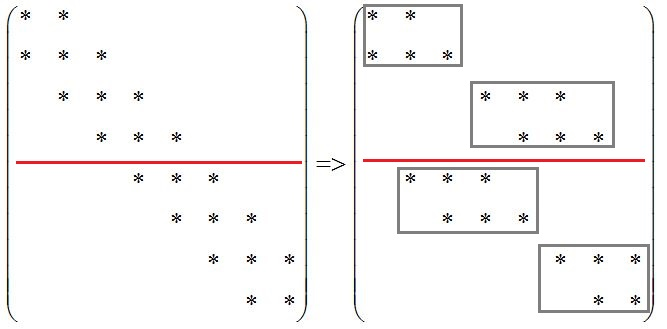
\includegraphics[width=4in]{Images/permutation}
\end{minipage}
\caption{Re-ordering the banded matrix}
\label{fig:permutation}
\end{figure}
 
 In Figure \ref{quality} we consider different types of partitions, both in the inner and outer levels. We found that have more independent blocks resulted in faster implementation of Kaczmarz. We also found that more partitions, i.e. taking 4 partitions: $$A = \begin{pmatrix} A_1^T  \\A_2 ^T \\ A_3^T \\ A_4^T \end{pmatrix} $$ instead of 2 partitions is slower. 
 
  Furthermore, it has been proven that the optimal value of $\omega$ is 1.0 if we use two partitions, and $Q(1)$ has the minimal spectral radius. For these reasons we decided to use 2 outer partitions for our implementation. In this case the problem can be simplified as follows: $$(I-Q)x = Tf$$


\begin{figure}[ht]
\begin{centering}
%\begin{minipage}[b]{1\linewidth}
\includegraphics[width=6in]{Images/quality.jpg}
%\end{minipage}
\end{centering}
\caption{Speed for different partition types.}
\label{quality}
\end{figure}


%\begin{figure}[ht]
%\centering
%\begin{minipage}[b]{1.0\linewidth}
%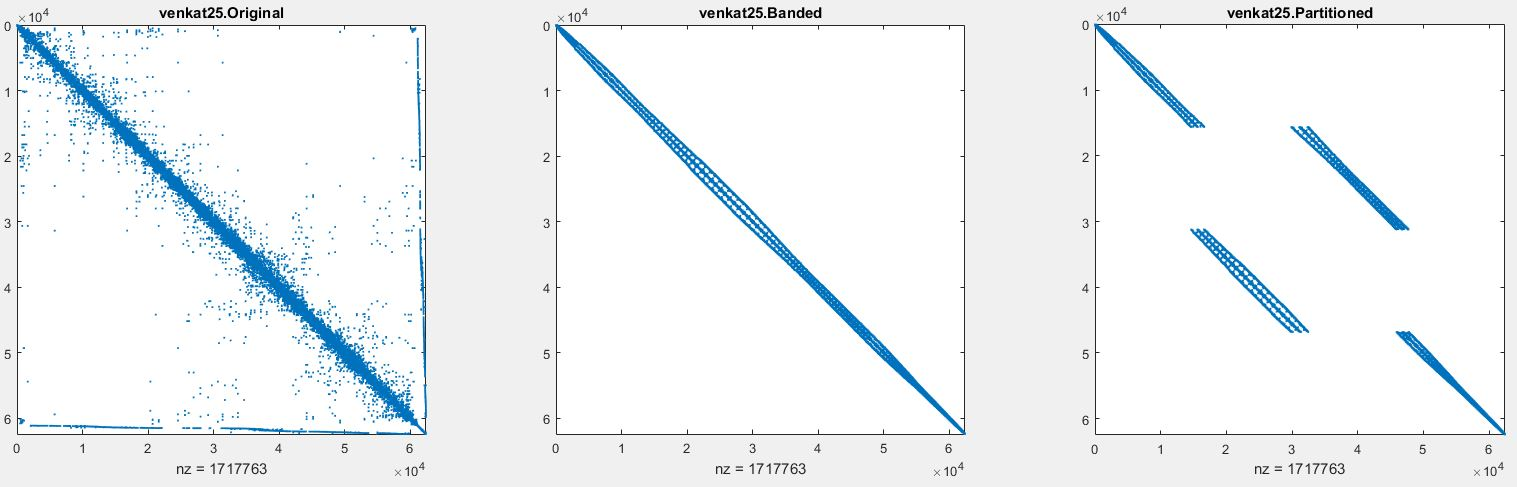
\includegraphics[width=4.8in]{Images/permute.jpg}
%\caption{$A$ is partitioned into 2 parts with several independent submatrices}
%\end{minipage}
%\end{figure}


%------------------------------------------------
%------------------------------------------------
% SYMMETRIZE KACZMARZ
% NEEDS SOME HELP
%------------------------------------------------
%------------------------------------------------
\subsection{Calculation of $c$}
To transform the system $Ax = f$ into solving the symmetric positive definite system $(I-Q)x = c$, we need to get the new right hand side vector $c$. Recall that we use $m=2$ partitions in our work. We let

 $$A = \begin{pmatrix} A_1^T \\ A_2^T \end{pmatrix}  $$ and we also partition the right hand size vector $$f^T = (f_1^T, f_2^T).$$
 
 For two partitions, if we expand $c = Tf$ to be:
 
 $$\textbf{Tf} = \begin{bmatrix} (I + (I-P_2)(I-P_1))(A_1^T)^+ && (I-P_1)(A_2^T)^+ \end{bmatrix} \begin{bmatrix} f_1  \\ f_2 \end{bmatrix}= c $$
 
 We see that in order to perform this we need to solve two pseudo inverse problems:
 
 $$\hat{f}_i = (A_i^T)^+f_i$$
 
 and whenever we see a product of the form $(I-P_i)u = v$ we are really performing a least squares operation involving the block $A_i$. We will discuss this least squares problem in more detail later.
 
Computing $c$ can be accomplished by solving a saddle point problem. In our implementation we spent some of our efforts trying to compute $c$, but due to time constraints and difficulties with other parts of our algorithm we were not able to ever correctly incorporate a proper computation of $c$ in our work. For this reason, for our code we generated a right hand side vector $c$ by setting $u$ to be the all ones vector, and then performing $c := (I-Q)\cdot u$ via a sequence of least squares operations. Then we were able to use our conjugate gradient framework to solve the system $(I-Q)x = c.$ 

In general for Kaczmarz we expect the time taken in running the CG scheme and calling the least squares function to be the bottleneck in our computations. So even though we were unable to properly generate the right hand side vector from a starting vector $f$, we chose to instead focus on the CG scheme and least squares framework in our implementation. 
 

\subsection{Least Squares Computations}
Recall that the new system we are dealing with is $(I-Q)x = c$, where $c = Tf$, and $$Q=(I-P_{1})(I-P_{2})(I-P_{1})$$
 with $P_{i}=A_{i}(A_{i}^{T}A_{i})^{-1}A_{i}^{T}$.

It is not stable to form $P_{i}$ directly since it will square the condition number of $A_{i}$, and at the same time will cost time in solving a system with the matrix $(A^{T}_{i}A_{i})$. Instead, given a vector $u$ we note that $v=(I-P_{j})u \Leftrightarrow \min\limits_{v}||u-A_{j}w||_{2}$. We therefore solve $\min\limits_{v}||u-A_{j}w||_{2}$ to obtain the vector $v$. 

%In PETSc, we use the CG method on the normal equations: $A_{j}^{T}A_{j}w=A_{j}^{T}u$. The parallel step is:
%        \begin{equation*}
%            \begin{split}
%                v&=\min\limits_{v}||u-A_{j}w||_{2}\Leftrightarrow \min\limits_{v_{i}}||u_{i}-A_{j,i}w_{i}||_{2},\\
%                v&^{T}=[v_{1}^{T},v_{2}^{T},...,v_{k}^{T}],\\
%                w&^{T}=[w_{1}^{T},w_{2}^{T},...,w_{k}^{T}].
%            \end{split}
%        \end{equation*}

Because of the way we have split our matrix, when we solve a least squares problem $(I-P_i)u = v$ we in theory can do so independently because $A_i$ is a matrix with many independent blocks. For proper parallel implementation, we would perform the following steps:

\begin{enumerate}
\item At the beginning of the algorithm, send different blocks of $A_i$ (for each sub matrix $i$) to different processors.
\item In each least squares computation, independently perform least squares operations on the blocks, and then gather the final result after the simultaneous, independent least squares operations.
\end{enumerate}

\subsubsection*{QR Factorizations}
One very effective way to compute the least squares problem in parallel is to use the QR factorization via Given's rotations on each independent block of each sub matrix $A_i$. The computation and storage of the QR factorization of the entire matrix $Q$ would be extremely expensive. However, because $A_i$ is made up of independent diagonal blocks that are all very small in size, we can perform QR factorizations of each of these blocks with great success.

There are two clear benefits of using the QR factorization on the independent sub blocks of $A_i$. First of all, we can find this factorization simultaneously for each block of $A_i$ at the very beginning of the algorithm, then in all future calls to our least squares function we can use the factorization without needing to recompute it. Secondly, the storage required for the factorization of the blocks is very small in comparison with the overall system.

\subsubsection*{Difficulties}

Unfortunately in our project we were not able to make full use of the parallelism that is theoretically possible by the Kaczmarz framework. Our difficulty was that splitting up a parallel matrix $A_i$ into independent pieces is extremely difficult in PETSc. This causes a number of issues in our final code, including the following:

\begin{itemize}
\item We cannot be sure that the blocks are perfectly split up among different processors, since PETSc assigns rows automatically by itself without our control.
\item Even though we have multiple processors at work on a least squares problem, the least squares computation is still performed globally on the entire sub matrix $A_i,$ rather than simultaneously on independent blocks of $A_i$.
\item We are unable to factorize pieces of $A_i$ ahead of time to save time in later calls to our sequential least squares algorithm
\end{itemize}

With a better knowledge of PETSc these problems could be remedied, but time constraints rendered it impossible to master the software enough so that we could reach the full potential of the Kaczmarz framework.

\subsubsection{Attempt to Improve Speed by LSQR}

In the end, in order to solve the least squares problem, we implemented LSQR. LSQR is an iterative method for solving $Ax = b$ where $A$ is large, sparse, and overdetermined. It is equivalent at each iteration to CG. 


\begin{algorithm}
\caption{LSQR}
\begin{algorithmic}[1]
%\Require{$P_1$ an initiator matrix; $n$, where we want to use $P_n$}
\State{$\beta_{1}u_{1}=b, \alpha_{1}v_{1}=A^{T}u_{1}, w_{1}=v_{1}, x_{0}=0, \bar{\phi_{1}}=\beta_{1},\bar{\rho_{1}}=\alpha_{1}$}
\For{$i = 1,2,3,\cdots$}
\State{Bidiagonalization:}
\State{$\beta_{i+1}u_{i+1}=Av_{i}-\alpha_{i}u_{i}$}
\State{$\alpha_{i+1}v_{i+1}=A^{T}u_{i+1}-\beta_{i+1}v_{i}$}
\State{Orthogonal Transformation:}
\State{$\rho_{i}=\sqrt{(\bar{\rho_{i}^2}+\beta_{i+1}^2)}$}
\State{$c_{i}=\bar{\rho_{i}}/\rho_{i},$}
\State{$s_{i}=\beta_{i+1}/\rho_{i},$}
\State{$\theta_{i+1}=s_{i}\alpha_{i+1},$}
\State{ $\bar{\rho_{i+1}}=-c_{i}\alpha_{i+1},$}
\State{$\phi_{i}=c_{i}\bar{\phi_{i}},$}
\State{$\bar{\phi_{i+1}}=s_{i}\bar{\phi_{i}}.$}
\State{Update x:}
\State{$x_{i}=x_{i-1}+(\phi_{i}/\rho_{i})w_{i},$}
\State{$w_{i+1}=v_{i+1}-(\theta_{i+1}/\rho_{i})w_{i}.$}
\EndFor

\end{algorithmic}
\end{algorithm}

    \begin{figure}[htbp]
    \begin{center}
        %\begin{minipage}[b]{0.8\linewidth}
            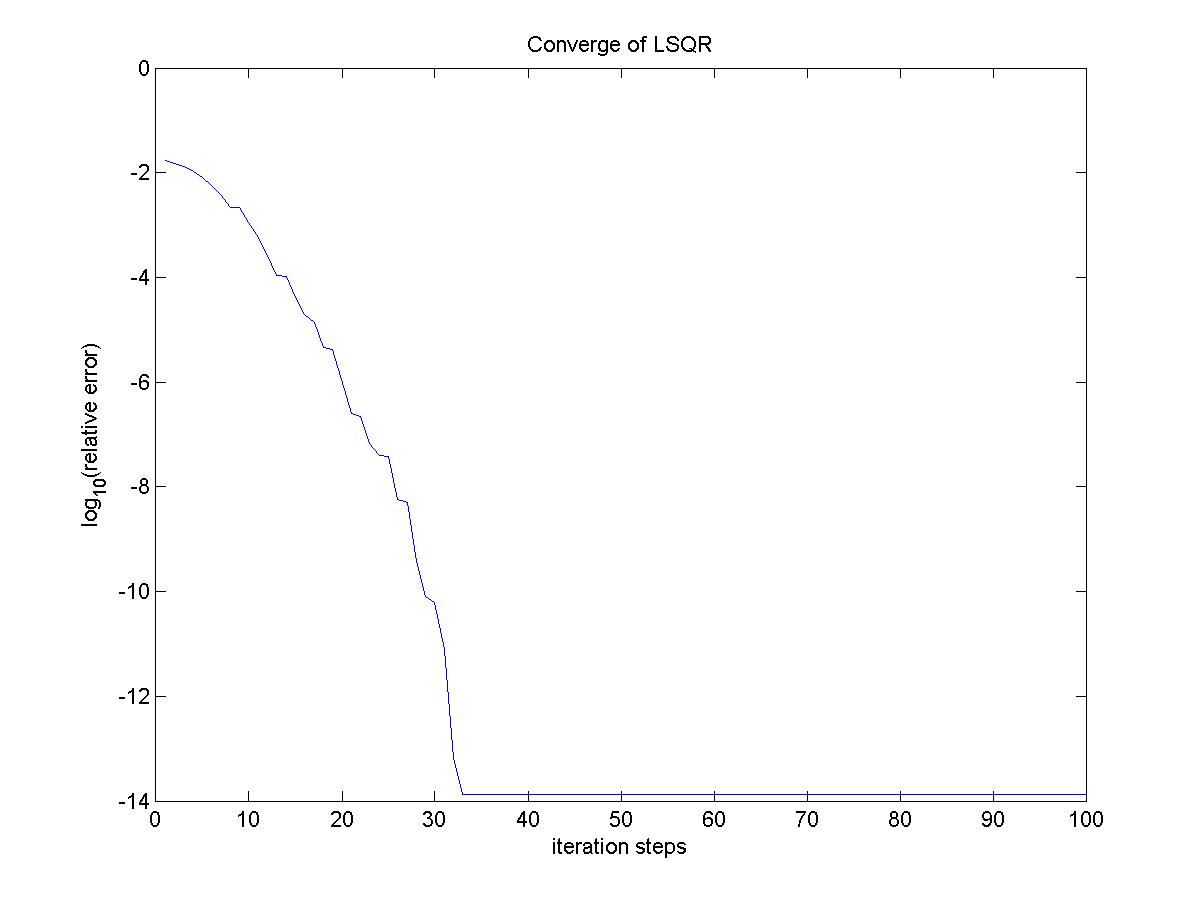
\includegraphics[width=3in]{Images/LSQR}
        %\end{minipage}
        \caption{Convergence of LSQR}
        \label{fig:LSQR}
        \end{center}
    \end{figure}
    
We had hoped that using this method and truncating the number of iterations used in the least squares calculations would allow us to obtain good overall results for our Kaczmarz algorithm. Note the plot of the convergence of the LSQR method in Figure \ref{fig:LSQR}. We can see that the algorithm mostly converges in the first several iterations, so we hoped that by truncating the number of steps taken we would make the least squares computation faster without harming the accuracy too much. We know that Krylov subspace methods are robust against poor matrix-vector products, so the hope was that our outer CG scheme would still progress towards an accurate overall solution of $(I-Q)x = c.$ . However, our final results are still far from satisfactory in terms of accuracy if we truncate the computations too much.

One thing we tried was to increase the maximum number of inner LSQR iterations used as the number of outer CG scheme iterations increased. We did this to try to find a balance between speed and accuracy. However, to achieve any type reasonable accuracy for our larger test cases, we did eventually need to make the iterative least squares method run for many iterations (over 100 for each least squares computation). This leads to very slow runtimes. We provide our results in a later section.

 %------------------------------------------------
%------------------------------------------------
% ACCELERATION VIA CG
%MAYBE NEEDS SOME HELP
%------------------------------------------------
%------------------------------------------------

 \subsection{Acceleration via the CG Method}
As stated previously, since $(I-Q)$ is symmetric positive definite, we accelerate solving $(I-Q)x = Tf$  using the conjugate gradient method. This is the framework of our entire algorithm. The outline follows:

\vspace{.2in}
 \noindent \textbf{Step 1} : $x_0 = c$ \\
\hspace{.5in} Compute $r_0 = Tf - \boxed{(I-Q)c} = Qc$\\
\hspace{.5in} Set $p_0 = r_0, i = 0$ \\
\textbf{Step 2}:  Compute: \\
\hspace{.5in} $\alpha_i = (r_i, r_i)/(p_i,\boxed{(I-Q)p_i})$ \\
\hspace{.5in} $ x_{i+1} = x_i + \alpha_i p_i $ \\
\hspace{.5in} $\beta_i = (r_{i+1}, r_{i+1})/(r_i, r_i) $ \\
\hspace{.5in} $p_{i+1} = r_{i+1} + \beta_i p _i $ \\
\textbf{Step 3}: If convergence criterion is satisfied, terminate the iterations; else set $i = i+1$ and return to Step 2.

 We can take a convergence criterion as : $$ \frac{ ||r_i||}{||r_0||} \leq \epsilon$$


The boxed out portions in our framework are very important. Remember that whenever we see: $$(I - Q) u$$ for any vector $u$, we really mean to solve multiple least squares problems:
$$(I-Q) u = (I-P_1)(I-P_2)(I-P_1) u $$
$$(I-P_i) u \Rightarrow \text{min}_{v} ||u-A_i w|| $$

 %------------------------------------------------
%------------------------------------------------
% LAST SECTION: RESULTS
%------------------------------------------------
%------------------------------------------------

\section{Results and Conclusions}

\subsection{Results}

We will now discuss the results of our parallel solver. Because of our slow least squares computations, we did not reach a very low tolerance for any of our test cases. For this reason we chose to simply truncate our CG loop at 100 iterations and report the runtime and the tolerance attained by this point. The results are given in table $\ref{tab:badresults}$.

\begin{table}
\begin{center}
\begin{tabular}{| l | l | c  c | c  c |}
\hline
                         &                & Our Parallel & Solver & Krylov & ILU\\
                          \hline
    matrix           & size         &  tol achieved & time (s)     &  num-its & time (s)        \\
 \hline
 lns                   & 131             &     $7.5E{-03}$   &         5.6  & \color{red} $\times$  &  \color{red} $\times$\\
 Jac2-db            & 21,982     &   $2.0E{-04}$     &    283    &  \color{red} $\times$  & \color{red} $\times$ \\
 venkat25         & 62,424      & $2.5E{-03}$      &     874  & 374                   & 14.17 \\
 stomach          & 213,360    &   $2.1E{-06}$    & 194 & 16                   & 2.21 \\
 atmosmodd     & 1,270,432 &  $3.0E{-03}$     &7100 &  266                   & 130.72 \\
 \hline

\end{tabular}
\end{center}
\caption{Runtimes of our algorithm (100 iterations of CG) in comparison with GMRES}
\label{tab:badresults}
\end{table}

To find a benchmark of how our method performed, we compared with a Krylov Subspace method. The implementation of this consisted of first using the MC64 software to re-order the matrix. This software finds a permutation which brings non-zeros to the diagonal. Once this permutation is used, then we called a Krylov Subspace method with ILU pre-conditioner in PETSc. The Krylov subspace method used is GMRES.

Note that the ILU preconditioner fails for some of our data. The reason for this could be that the eigenvalues of these matrices are distributed too much across the positive and negative spectrum. The ILU preconditioner is not well equipped to handle these so called ``highly indefinite'' matrices. Table \ref{tab:MC64} shows which of our data failed with this method.
\begin{table}
\begin{center}
\begin{tabular}{| l | l | c |}
\hline
matrix             & size        & Converged? \\
\hline
lns                  & 131         &    \color{red} $\times$  \\
std1-Jac2-db  & 21,982    & \color{red}  $\times$  \\
venkat25        & 62,424     & \color{green} \Checkmark   \\
stomach         & 213,360   &  \color{green}  \Checkmark  \\
atmosmodd    & 1,270,432 &  \color{green} \Checkmark  \\
\hline
\end{tabular}
\end{center}
\caption{ILU preconditioner}
\label{tab:MC64}
\end{table}

We note that the one success of our algorithm was its ability to make progress in solving the first few test cases where we failed to converge for GMRES. We see that the framework of our algorithm is good for solving these difficult systems, though runtimes are terrible for reasons already addressed.

\subsection{Conclusions}
In conclusion, it was a mistake to use PETSc. PETSc is better for high level implementation, not for optimization and efficiency. PETSc was also not well suited specifically for grabbing the exact sub-matrices that we needed in order to call the parallel Least Squares. 

In the end we tried to salvage our project by implementing LSQR, but even with this attempt we did not obtain the desired outcome. If we had left PETSc out of our project we know our results would have been even better.

\nocite{KamathSameh1988,GallopoulosPhilippeSameh2016,Paige,HSL}

\newpage

\bibliography{Ref}
\bibliographystyle{plain}

\end{document}


